WSDL ist eine XML-basierte Sprache zur Beschreibung von Web-Services.
Sie beschreibt die Schnittstelle des Web-Services, nicht aber den Web-
Service selbst. Neben der Methodenspezifikation beinhaltet sie auch technische
Daten, wie die eigentliche Lage des Dienstes und an welche Transportprotokolle
er gebunden ist.

Obwohl WSDL 2.0 am 23. May 2007  ver�ffentlicht wurde, wird in dieser Arbeit WSDL 1.1 \cite{W3C2001} verwendet.  
Der Grund hierf�r ist, dass die BPEL 2.0, um die es in dieser Arbeit in erster Linie geht, auch noch auf WSDL 1.1 aufsetzt.

Abbildung \ref{fig:wsdlStructur} zeigt die Struktur eines WSDL-Dokuments.
Die Elemente in einem WSDL-Dokument lassen sich in abstrakte Definitionen
und konkrete technische Beschreibungen zu diesen Definitionen unterteilen. 
F�r die sprach- und plattformunabh�ngige Beschreibung
der Schnittstelle (Datentypen, Operationen und Nachrichten) sind die abstrakten Elemente zust�ndig: $<$types$>$-, $<$message$>$- und $<$portType$>$.
Die konkreten technischen Details (wo die Services sich befinden und wie sie aufgerufen werden k�nnen) werden durch die Elemente $<$binding$>$ und $<$service$>$ definiert.  Die konkreten Definitionen referenzieren
dabei stets abstrakte Definitionen. Das bedeutet, dass zu einer abstrakten
Definition mehrere konkrete Implementierungen  existieren k�nnen. Damit besteht die M�glichkeit, einen Service an mehreren Stellen verf�gbar zu machen und die Verwendung verschiedener Kommunikations- und Transportprotokolle zu erm�glichen. Im Folgenden werden die Elemente eines WSDL-Dokumentes einzeln beschrieben und n�her erl�utert.


\begin{figure}[htbp]
	\centering
		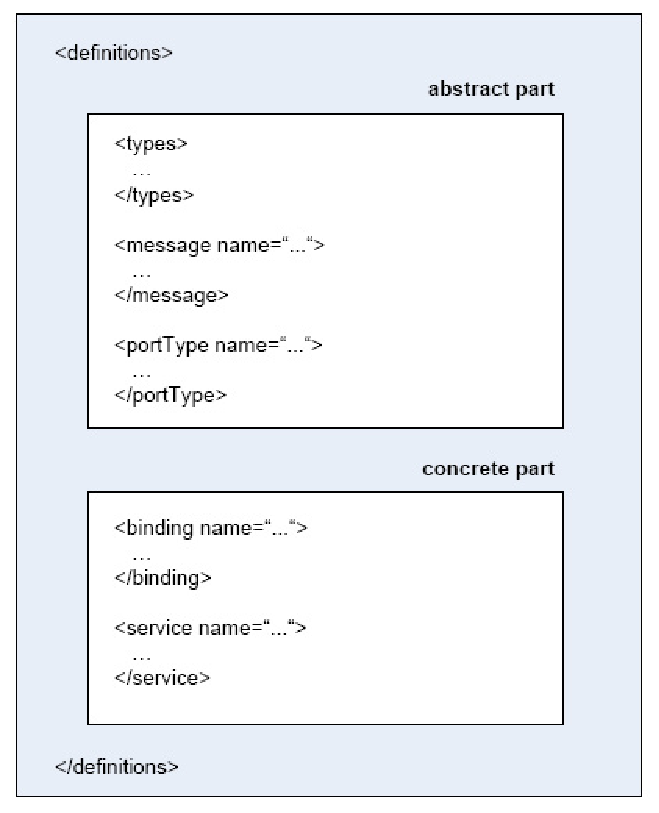
\includegraphics[width=0.42\textwidth]{bilder/wsdlStructur.pdf}
		\caption{WSDL-Dokumentformat}
	\label{fig:wsdlStructur}
\end{figure}

\textbf{$<$definitions$>$} ist das Wurzelelement des WSDL-Dokuments. Es enth�lt den Namen des Services, Namespaces f�r den Service selbst und f�r die verwendeten Standards.

\textbf{$<$types$>$} enth�lt Definitionen f�r eigene Datentypen. Standardm��ig werden die Datentypen aus des XML-Schema-Spezifikation verwendet. Die Flexibilit�t der XML-Schemas, die sprachun\-abh�ngig und plattformneutral sind, erlaubt es, in WSDL die Besonderheiten bestehender Programmiersprachen oder Datenaustauschstandards abzubilden.


\textbf{$<$message$>$}  fasst die definierten Typen zu abstrakten unidirektionalen Nachrichten zusammen.

\textbf{$<$portType$>$} beschreibt die Schnittstelle des Services, die eine oder mehrere
Operationen zusammen fasst. Diese ordnen der Operation
die Ein- und Ausgabeparameter zu und legen damit das Nachrichtenaustauschmuster fest.

\textbf{$<$binding$>$} definiert die vom Web Service verwendeten Kommunikationsprotokolle und Nachrichtenformate. Die meist benutzten Protokolle sind SOAP, HTTP GET/POST. 

\textbf{$<$service$>$} stellt aus einem oder mehreren ports einen Dienst zusammen.
Ein port ordnet dem Binding einen bestimmten Endpunkt zu. Die genaue Definition h�ngt vom verwendeten Transportprotokoll ab.




